\section{Introdução ao LibreOffice Writer}

\begin{frame}{Introdução}
	\begin{block}{}
		\begin{itemize}
			\item O LibreOffice é um pacote de \textbf{produtividade de escritórios} totalmente \textbf{funcional} e disponível \textbf{gratuitamente}.
			\item Ele é baseado no OpenDocument (ODF), um padrão de formatos \textbf{abertos} que está sendo adotado por governos do mundo inteiro como \textbf{necessário} para a publicação de documentos.
			\item O LibreOffice também pode \textbf{abrir} e \textbf{salvar documentos} em muitos outros formatos, incluindo aqueles utilizados por várias versões do \textbf{Microsoft Office}.
		\end{itemize}
	\end{block}

	\centering
	
\includegraphics[width=0.45\linewidth]{Figuras/Ch04/fig1.2}

	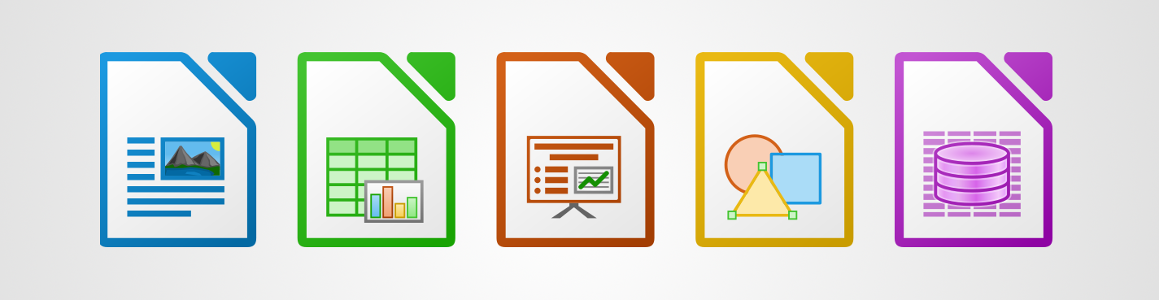
\includegraphics[width=0.6\linewidth]{Figuras/Ch04/fig1.1}
\end{frame}


\begin{frame}{Introdução}
	\begin{block}{Vantagens do LibreOffice}
		\begin{itemize}
			\item \textbf{Sem taxas de licenciamento:} o LibreOffice é \textbf{livre} para qualquer um usá-lo e distribuí-lo sem custos.
			\item \textbf{Software livre:} você pode distribuir, copiar e modificar o software o quanto quiser.
			\item \textbf{Multiplataforma:} o LibreOffice roda em várias arquiteturas de hardware e múltiplos sistemas operacionais, como o Microsoft Windows, Mac OS X e Linux.
			\item \textbf{Extenso suporte a idiomas:} a interface de usuário do LibreOffice, incluindo ortografia, hifenização e dicionários de sinônimos, está disponível em mais de 100 línguas e dialetos.
		\end{itemize}
	\end{block}
\end{frame}


\begin{frame}{Introdução}
	\begin{block}{Vantagens do LibreOffice}
		\begin{itemize}
			\item \textbf{Interface de usuário consistente:} todos os componentes possuem uma aparência semelhante, o que faz com que sejam fáceis de usar e controlar.
		\end{itemize}
	\end{block}

	\centering
	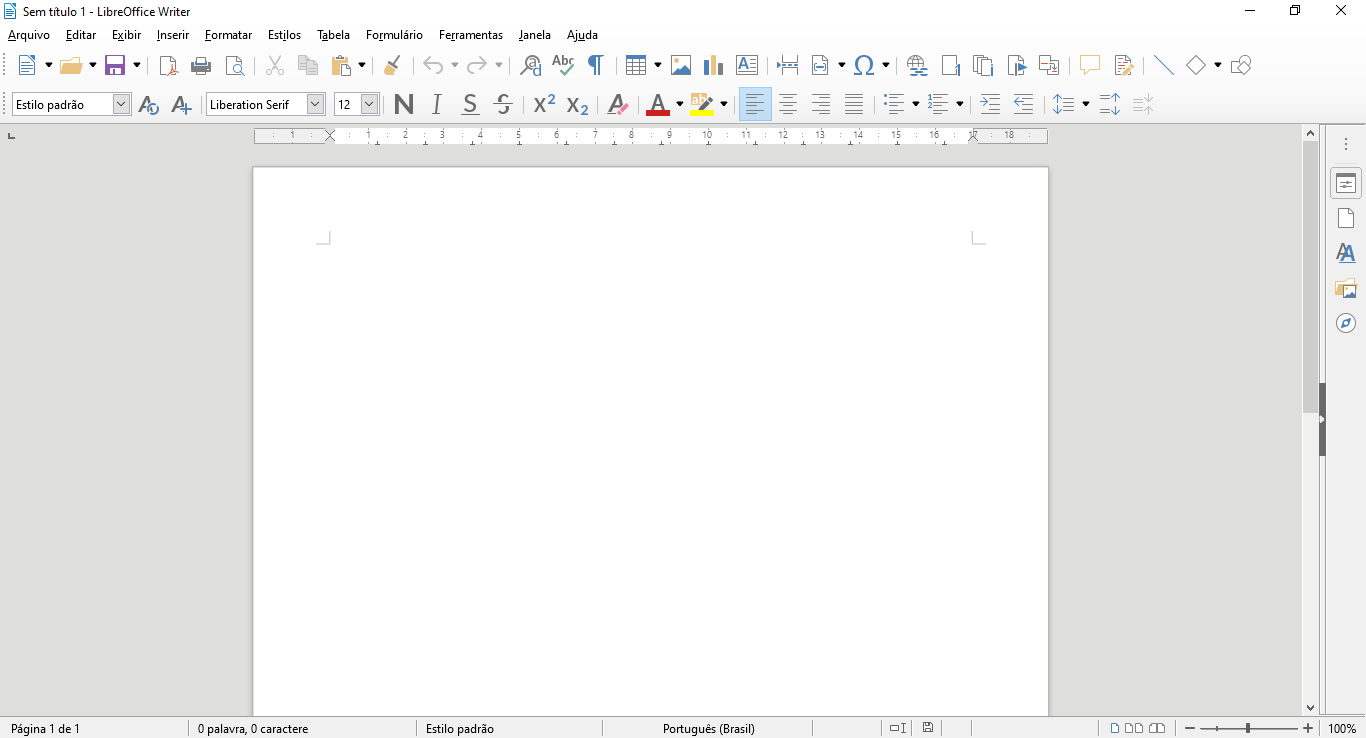
\includegraphics[width=0.8\linewidth]{Figuras/Ch04/fig2}

\end{frame}


\begin{frame}{Introdução}
	\centering
	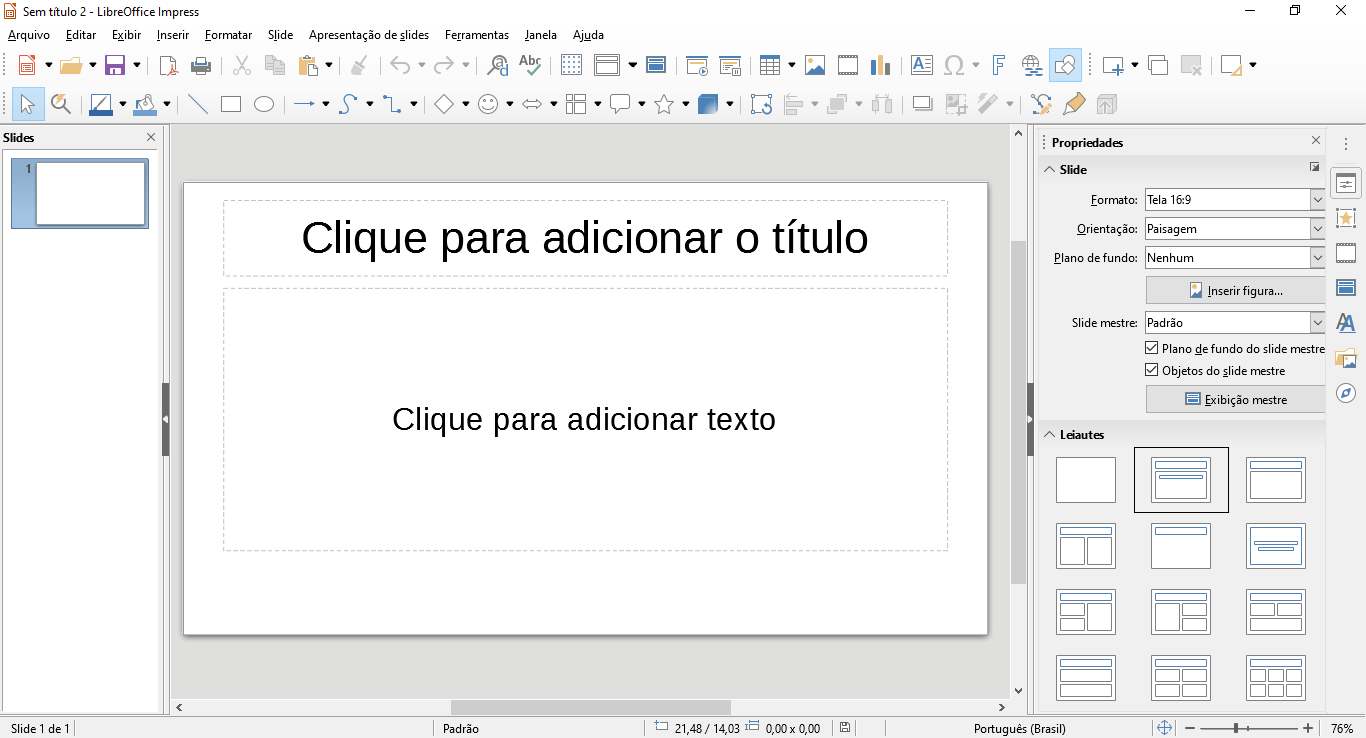
\includegraphics[width=1\linewidth]{Figuras/Ch04/fig3}
\end{frame}


\begin{frame}{Introdução}
	\centering
	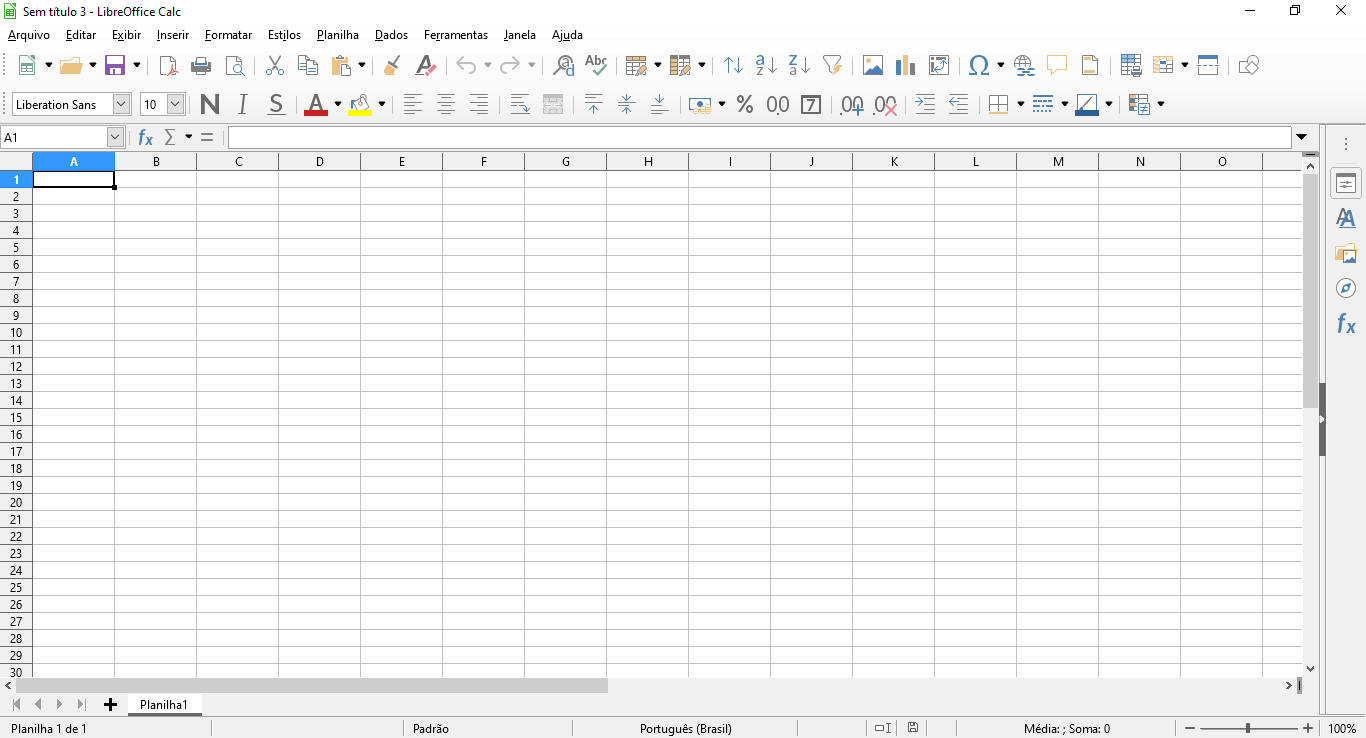
\includegraphics[width=1\linewidth]{Figuras/Ch04/fig4}
\end{frame}


\begin{frame}{Introdução}
	\begin{block}{Como conseguir uma cópia?}
		\begin{itemize}
			\item Versões do LibreOffice para Windows, Linux, e Mac OS X podem ser baixados de: \url{http://www.libreoffice.org/download}
			\item Você pode baixá-lo, também, utilizando um cliente, como o BitTorrent, no mesmo endereço.
		\end{itemize}
	\end{block}

	%	\centering
	%	\includegraphics[width=0.7\linewidth]{Figuras/Ch04/fig}
\end{frame}


\begin{frame}{LibreOffice Writer}
	\begin{block}{}
		\begin{itemize}
			\item O \textit{Writer} é uma ferramenta riquíssima para criação de cartas, livros, relatórios, jornais, cadernos e outros tipos de documentos.
			\item Você pode inserir \textbf{gráficos} e \textbf{objetos de outros componentes} dentro dos documentos do Writer.
			\item O Writer é capaz de exportar arquivos para os formatos HTML, XHTML, XML, Portable Document Format (PDF) da Adobe, e até para os formatos do Office.
			\item Ele também pode conectar-se ao seu programa de \textit{e-mail}.
		\end{itemize}
	\end{block}

	\centering
	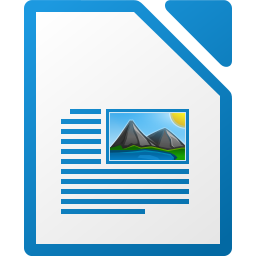
\includegraphics[width=0.25\linewidth]{Figuras/Ch04/fig1}
\end{frame}


\begin{frame}{LibreOffice Writer}
	\centering
	
\includegraphics[width=1\linewidth]{Figuras/Ch04/fig0}
\end{frame}


\begin{frame}{LibreOffice Writer}
	\centering
	
\includegraphics[width=0.9\linewidth]{Figuras/Ch04/fig0.1}
\end{frame}


\begin{frame}{Janela principal}
	\begin{block}{}
		\begin{itemize}
			\item As funções comuns incluem a \textbf{barra de menu} (1), a \textbf{barra ferramentas padrão} (2), a \textbf{barra de ferramentas de formatação} (3) no topo da janela e a \textbf{barra de status} (4) na parte de baixo.
		\end{itemize}
	\end{block}

	\centering
	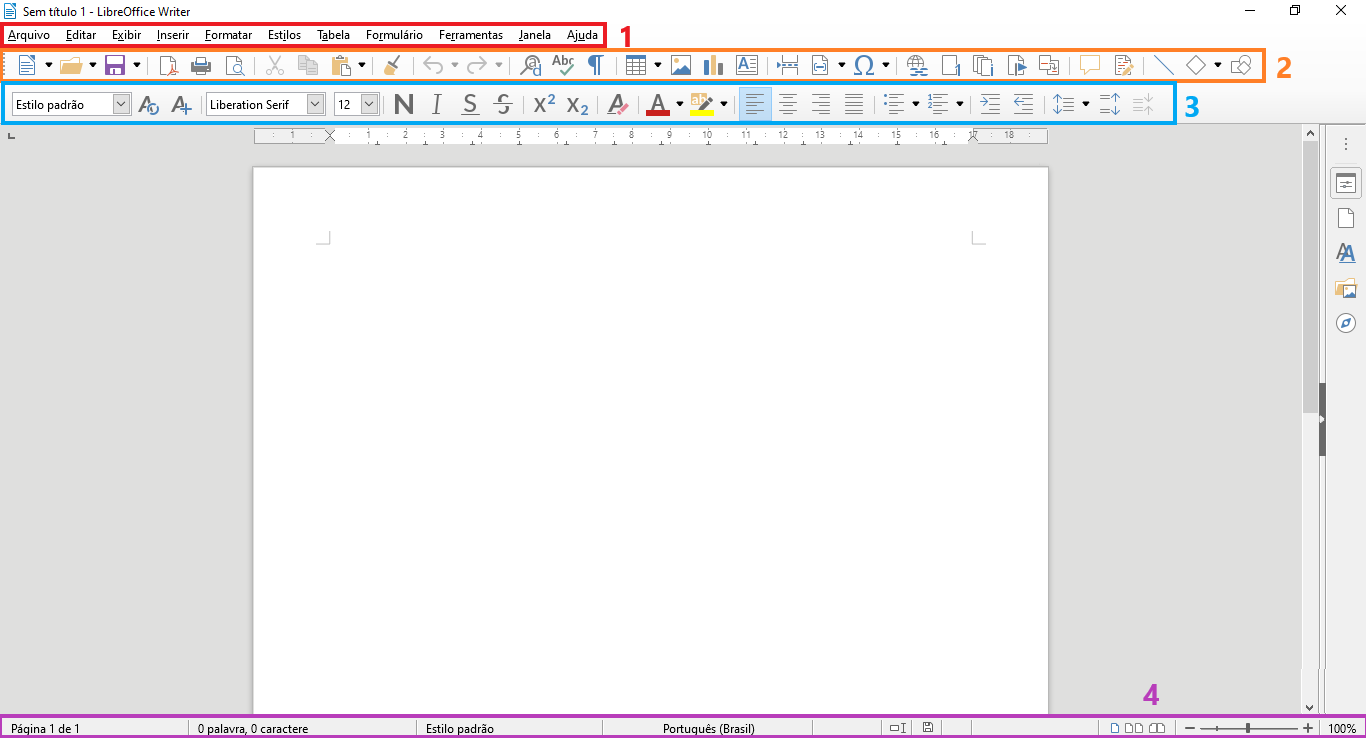
\includegraphics[width=0.9\linewidth]{Figuras/Ch04/fig5}
\end{frame}


\begin{frame}{Barra de menu}
	\begin{block}{}
		A barra de menu está localizada no alto da janela do LibreOffice, logo abaixo da barra de título.
	\end{block}

	\centerline{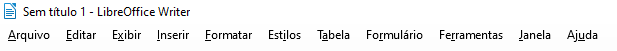
\includegraphics[width=1\linewidth]{Figuras/Ch04/fig6.1}}

	\begin{block}{}
		Quando você seleciona um dos itens listados a seguir, um submenu se abre para exibir os comandos.
	\end{block}

	\centerline{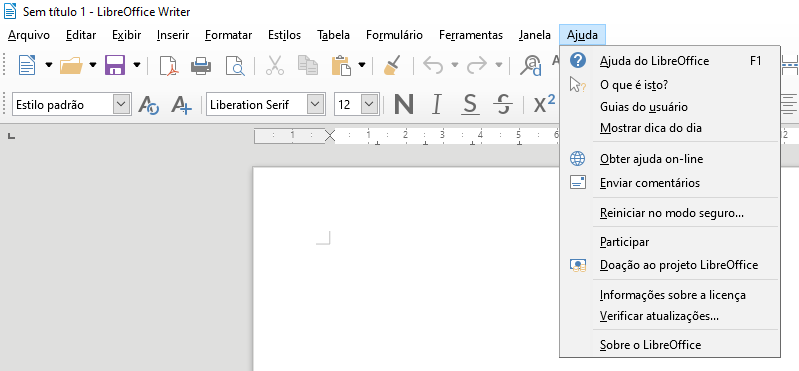
\includegraphics[width=0.7\linewidth]{Figuras/Ch04/fig6}}
\end{frame}


\begin{frame}{Barra de menu}
	\begin{block}{}
		\begin{itemize}
			\item \textbf{Arquivo:} contém os comandos que se aplicam a todo o documento, como Abrir, Salvar, e Exportar como PDF.
			\item \textbf{Editar:} contém os comandos para a edição do documento, tais como Desfazer, Localizar e Substituir, Recortar, Copiar e Colar.
			\item \textbf{Exibir:} contém comandos para controle da exibição do documento, como Zoom e Layout da Web.
			\item \textbf{Inserir:} contém comandos para inserção de elementos em seu documento, como Cabeçalho, Rodapé e Documento.
		\end{itemize}
	\end{block}
\end{frame}


\begin{frame}{Barra de menu}
	\begin{block}{}
		\begin{itemize}
			\item \textbf{Formatar:} contém comandos, como Estilos e Formatação e Autocorreção, para formatação do seu documento.
			\item \textbf{Tabela:} contém todos os comandos para inserir e editar uma tabela em um documento de texto.
			\item \textbf{Ferramentas:} contém funções como Ortografia e Gramática, Personalizar e Opções.
			\item \textbf{Janela:} contém comandos de exibição da janela.
			\item \textbf{Ajuda:} contém atalhos para os arquivos de Ajuda do LibreOffice, O que é isso? e informações sobre o programa.
		\end{itemize}
	\end{block}
\end{frame}


\begin{frame}{Barra de ferramentas}
	\begin{block}{}
		\begin{itemize}
			\item O LibreOffice possui dois tipos de barras de ferramentas: \textbf{encaixada} (fixa no lugar) e \textbf{flutuante}.
			\item As barras de ferramentas encaixadas podem ser movidas para posições diferentes ou alteradas para flutuantes, e barras flutuantes podem ser encaixadas.
		\end{itemize}
	\end{block}

	\centering
	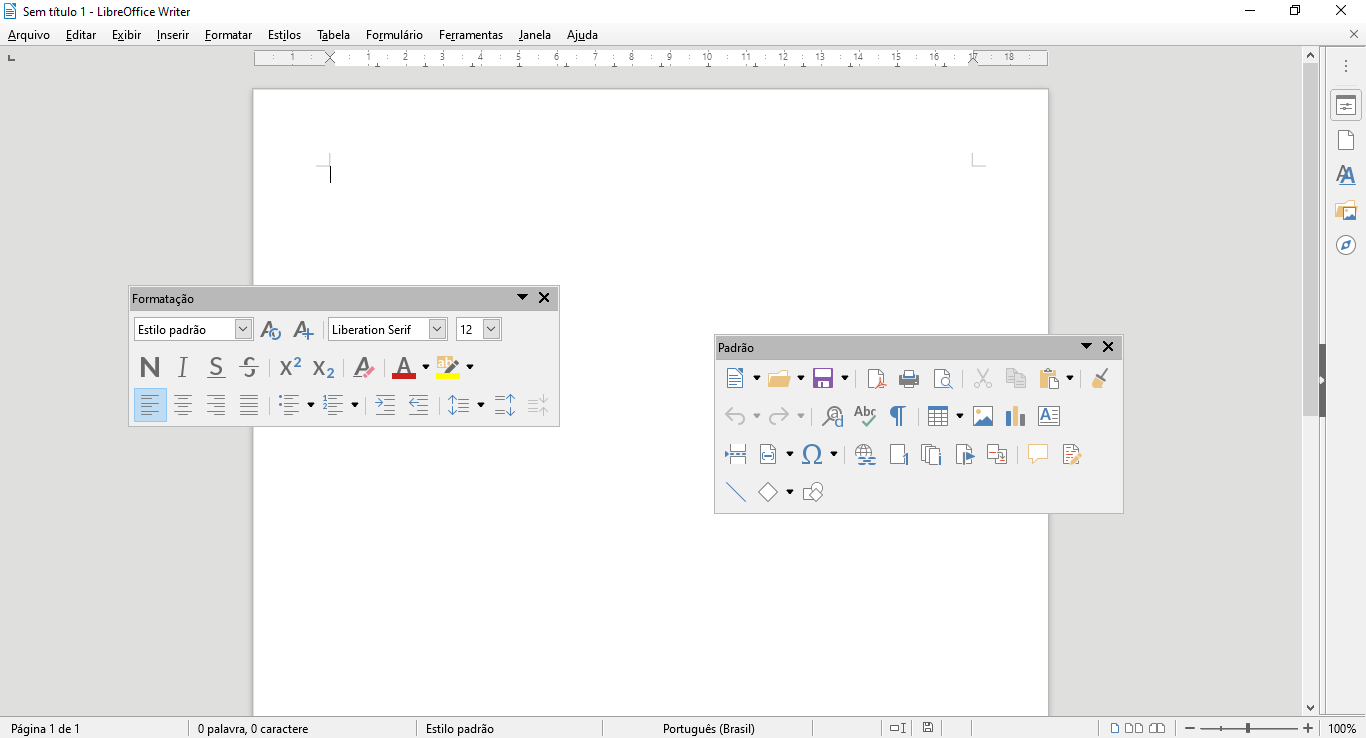
\includegraphics[width=0.75\linewidth]{Figuras/Ch04/fig7}

\end{frame}


\begin{frame}{Barra de ferramentas}
	\centering
	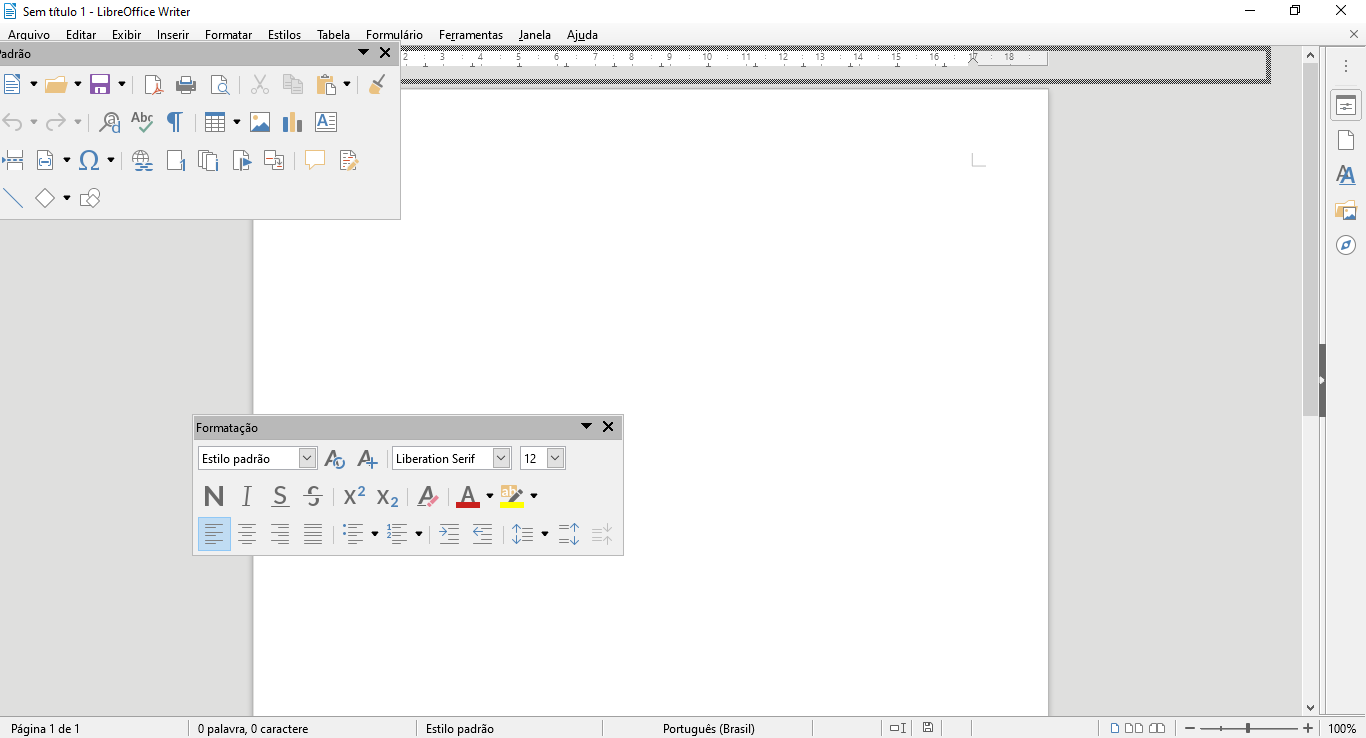
\includegraphics[width=1\linewidth]{Figuras/Ch04/fig8}
\end{frame}


\begin{frame}{Barra de ferramentas}
	\begin{block}{}
		\begin{itemize}
			\item Em uma instalação padrão do LibreOffice, a barra de ferramentas superior, encaixada logo abaixo da barra de Menu, é chamada \textbf{barra de ferramentas padrão}.
			\item A Barra de ferramentas padrão é a mesma em todas as aplicações do LibreOffice.
		\end{itemize}
	\end{block}

	\bigskip

	\centering
	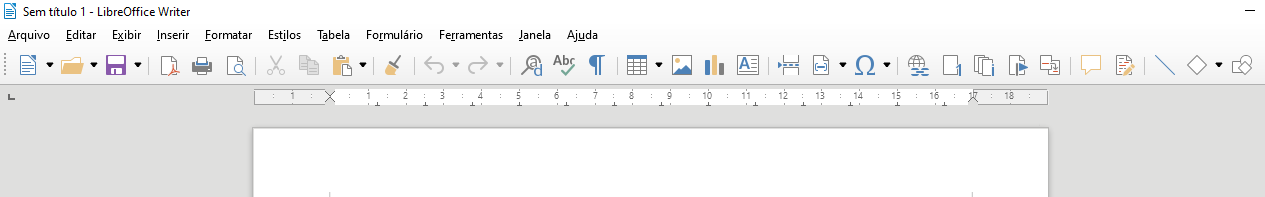
\includegraphics[width=1\linewidth]{Figuras/Ch04/fig9}
\end{frame}


\begin{frame}{Barra de ferramentas}
	\begin{block}{}
		\begin{itemize}
			\item A segunda barra de ferramentas no topo, em uma instalação padrão do LibreOffice, é a \textbf{barra de formatação}.
			\item É uma barra sensível ao contexto que mostra as ferramentas mais importantes, de acordo com a posição do cursor ou com a seleção.
			\item Por exemplo, quando o cursor está sobre um gráfico, a barra de formatação oferece ferramentas para a formatação de gráficos; quando o cursor está em um texto, as ferramentas são as de formatação de texto.
		\end{itemize}
	\end{block}

	\medskip

	\centering
	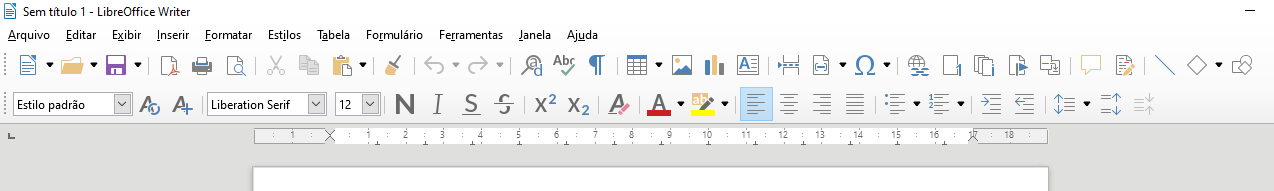
\includegraphics[width=1\linewidth]{Figuras/Ch04/fig10}
\end{frame}


\begin{frame}{Exibir ou ocultar barra de ferramentas}
	\begin{block}{}
		\begin{itemize}
			\item Para \textbf{exibir ou ocultar} barras de ferramentas, vá no menu Exibir > Barra de ferramentas e clique sob o nome da barra de ferramentas na lista suspensa.
			\item Uma barra de ferramentas ativa exibe uma marca verificação ao lado do seu respectivo nome.
			\item Barras de ferramentas criadas a partir de paletas de ferramentas não serão listadas no meu Exibir.
		\end{itemize}
	\end{block}

	\centering
	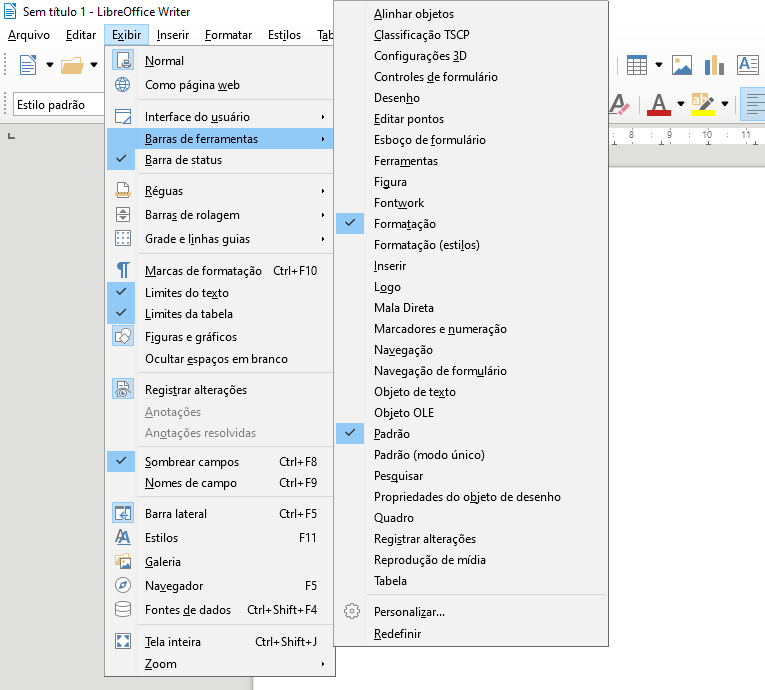
\includegraphics[width=0.5\linewidth]{Figuras/Ch04/fig11}
\end{frame}


\begin{frame}{Submenus e paletas de ferramenta}
	\begin{block}{}
		\begin{itemize}
			\item Ícones da barra de ferramentas com um pequeno triângulo à direita exibem submenus, paletas de ferramenta e outros meios de seleção de itens, dependendo do ícone.
		\end{itemize}
	\end{block}

	\centering
	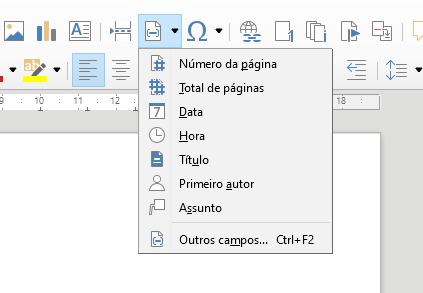
\includegraphics[width=0.7\linewidth]{Figuras/Ch04/fig12}
\end{frame}


\begin{frame}{Submenus e paletas de ferramenta}
	\begin{block}{}
		\begin{itemize}
			\item Paletas de ferramenta podem se tornar barras de ferramentas flutuantes (basta arrastar o tracejado).
		\end{itemize}
	\end{block}

	\bigskip

	\begin{minipage}{0.49\linewidth}
		\centering
		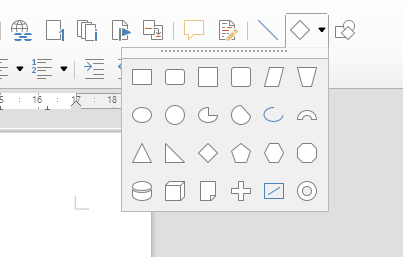
\includegraphics[width=1\linewidth]{Figuras/Ch04/fig13}
	\end{minipage}\hfill
	\begin{minipage}{0.49\linewidth}
		\centering
		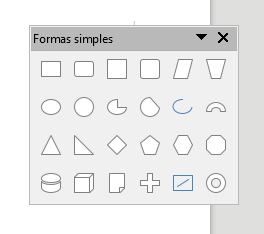
\includegraphics[width=1\linewidth]{Figuras/Ch04/fig14}
	\end{minipage}
\end{frame}


\begin{frame}{Barra de ferramentas flutuantes}
	\begin{block}{}
		\begin{itemize}
			\item O LibreOffice inclui diferentes \textbf{barras de ferramentas adicionais}, que por padrão aparecem como barras de ferramentas flutuantes conforme a posição atual do cursor ou seleção.
			\item Algumas dessas barras de ferramentas adicionais são sensitivas ao contexto e aparecerão automaticamente dependendo da posição do cursor.
			\item Por exemplo, quando o cursor está em uma tabela, a barra de ferramentas Tabela aparece, e quando o cursor está em uma lista numerada ou de marcadores, a barra de ferramentas Marcadores e Numeração aparece.
		\end{itemize}
	\end{block}
\end{frame}


\begin{frame}{Barra de ferramentas flutuantes}

	\centering
	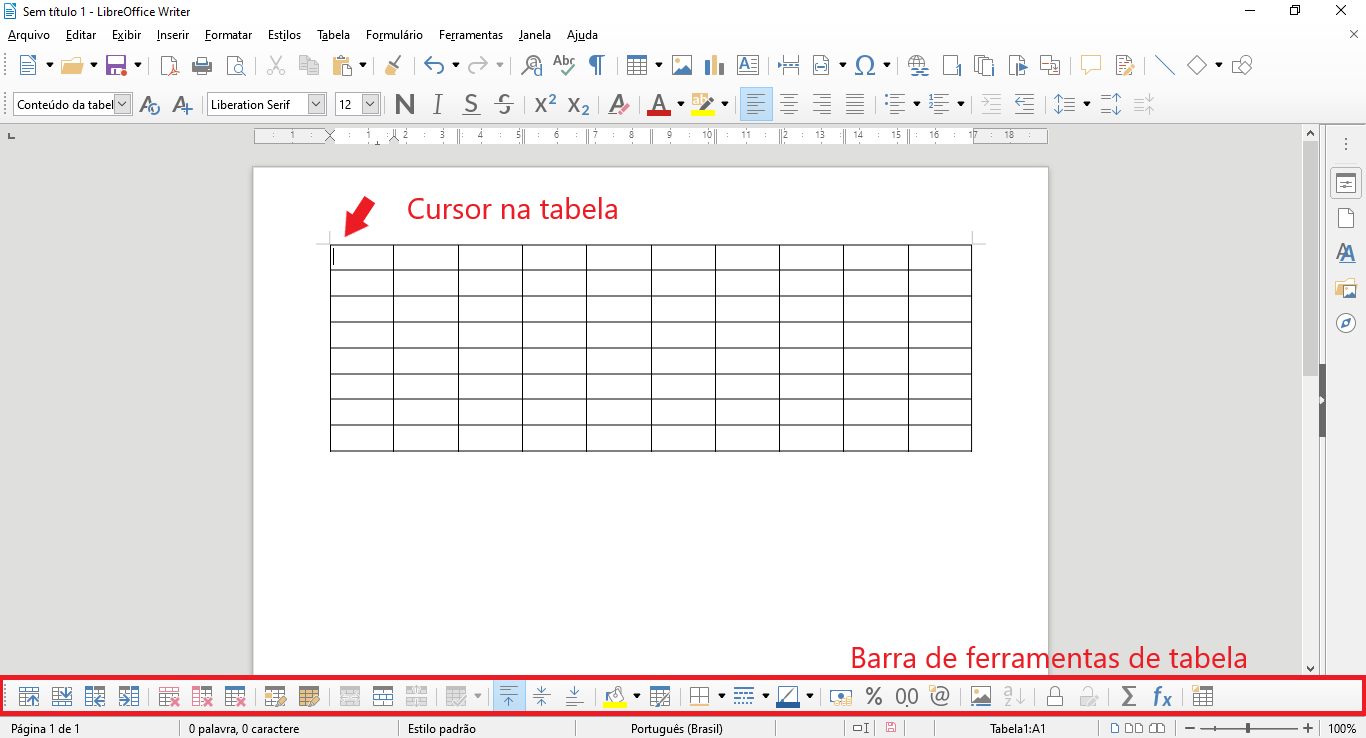
\includegraphics[width=1\linewidth]{Figuras/Ch04/fig15}
\end{frame}


\begin{frame}{Barra de ferramentas flutuantes}

	\centering
	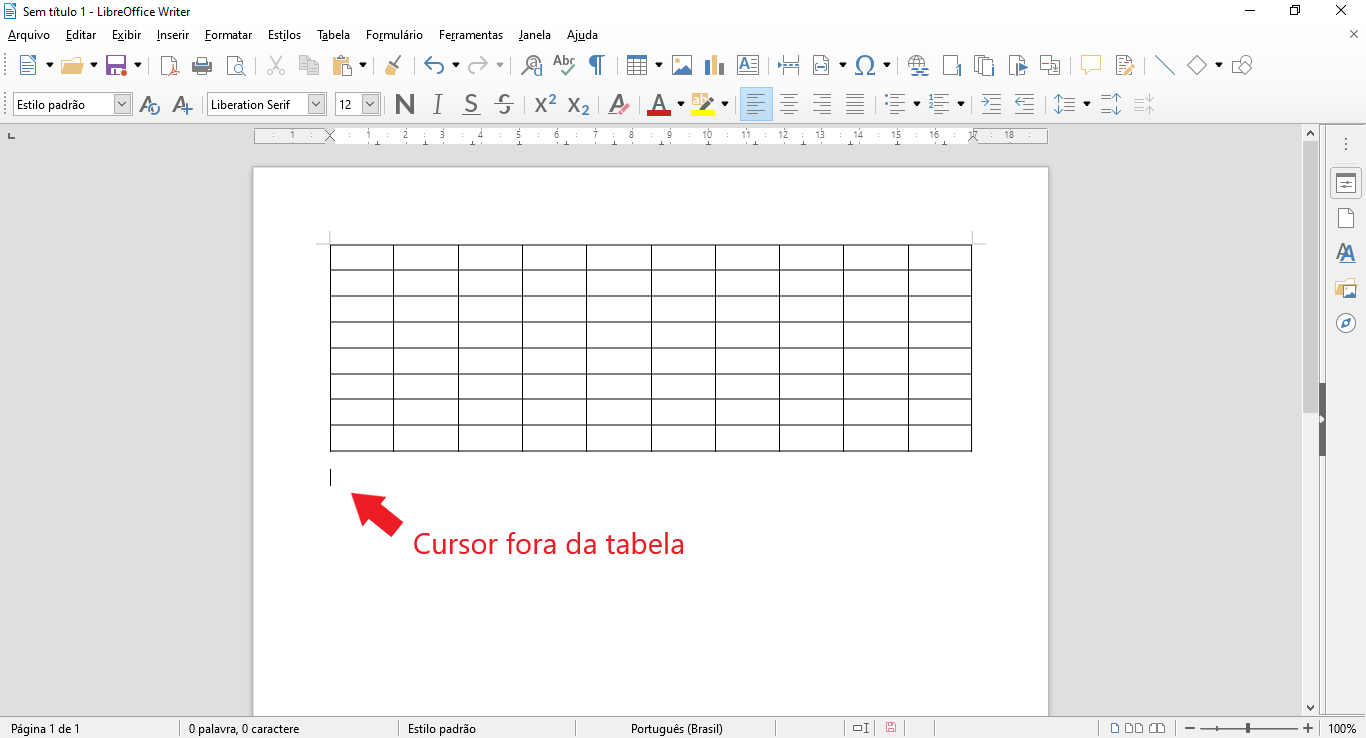
\includegraphics[width=1\linewidth]{Figuras/Ch04/fig16}
\end{frame}


\begin{frame}{Menu de contexto}
	\begin{block}{}
		\begin{itemize}
			\item Menus de contexto são uma forma de \textbf{acesso rápido para diversas funções}.
			\item Eles são abertos clicando com o botão direito em um parágrafo, gráfico ou outro objeto.
			\item Quando um menu de contexto é aberto, as funções ou opções disponíveis dependerão do objeto que estiver selecionado.
			\item Um menu de contexto pode ser a forma mais fácil para alcançar uma função, especialmente se você não está certo de onde ela está localizada nos menus ou barras de ferramentas.
		\end{itemize}
	\end{block}
\end{frame}


\begin{frame}{Menu de contexto}

	\begin{minipage}{0.49\linewidth}
		\centering
		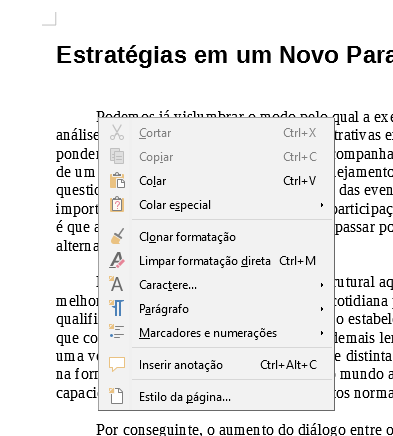
\includegraphics[width=1\linewidth]{Figuras/Ch04/fig17}
	\end{minipage}\hfill
	\begin{minipage}{0.49\linewidth}
		\centering
		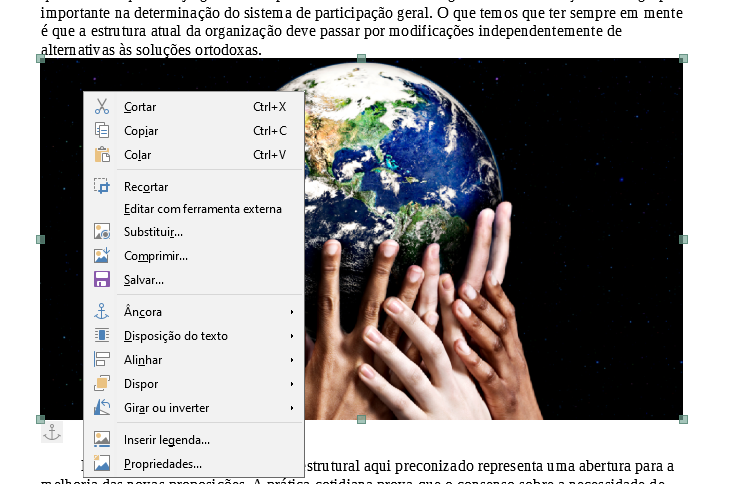
\includegraphics[width=1\linewidth]{Figuras/Ch04/fig18}
	\end{minipage}
\end{frame}


\begin{frame}{Barra de status}
	\begin{block}{}
		\begin{itemize}
			\item A barra de status está localizada na parte de baixo do espaço de trabalho.
			\item Ela fornece informação sobre o documento e formas convenientes para alterar de forma rápida alguns recursos.
			\item Isto é similar no Writer, Calc, Impress, mas cada componente do LibreOffice inclui alguns itens de componentes específicos.
		\end{itemize}
	\end{block}

	\bigskip

	\centering
	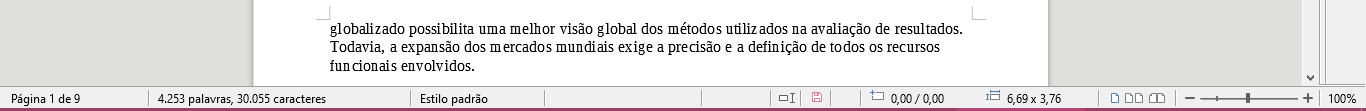
\includegraphics[width=1\linewidth]{Figuras/Ch04/fig19}
\end{frame}


\begin{frame}{Barra de status}
	\begin{block}{}
		\begin{itemize}
			\item \textbf{Página, planilha, ou número do slide e número da página:} mostra a página atual, planilha, ou número do slide e o número total de páginas, planilhas ou slides no documento. Clique nesse campo para abrir o Navegador.
			\item \textbf{Palavras e caracteres:} mostra o número total de palavras e caracteres no documento ou na seleção.
		\end{itemize}
	\end{block}

	\centering
	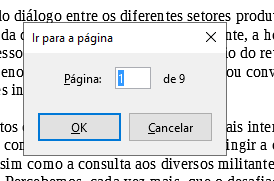
\includegraphics[width=0.55\linewidth]{Figuras/Ch04/fig20}
\end{frame}


\begin{frame}{Barra de status}
	\begin{block}{}
		\begin{itemize}
			\item \textbf{Barra de  da página ou design do desenho ou slide:} mostra o estilo atual da página ou desenho (design) do slide. Para editar a página atual ou o desenho (design) do slide, clique duas vezes nesse campo. Para escolher uma página de estilo diferente ou desenho de slide, clique com o botão direito e selecione uma opção da lista que se abre.
			\item \textbf{Idioma:} exibe o idioma atual do texto na posição do cursor atual.
		\end{itemize}
	\end{block}

	\centering
	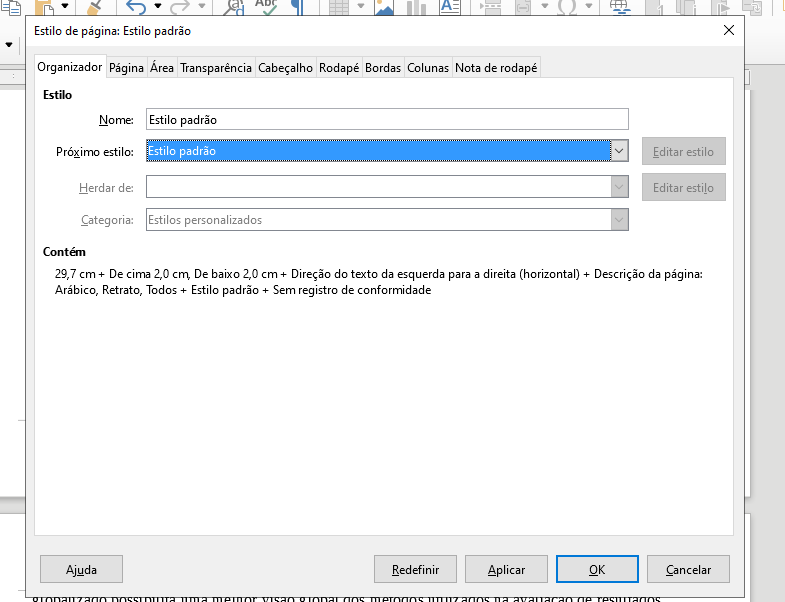
\includegraphics[width=0.45\linewidth]{Figuras/Ch04/fig21}
\end{frame}


\begin{frame}{Barra de status}
	\begin{block}{}
		\begin{itemize}
			\item \textbf{Alterações não salvas:} um ícone aparece aqui se as modificações do documento ainda não foram salvas.
			\item \textbf{Assinatura Digital:} se o documento foi assinado digitalmente, um ícone é mostrado aqui. Você pode clicar no ícone para assinar o documento, ou visualizar o certificado existente.
		\end{itemize}
	\end{block}

	\medskip

	\centering
	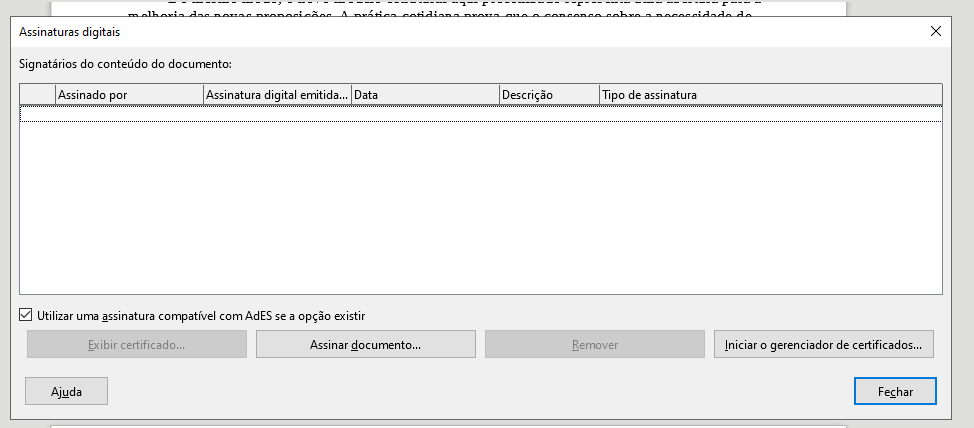
\includegraphics[width=0.8\linewidth]{Figuras/Ch04/fig22}
\end{frame}



\begin{frame}{Barra de status}
	\begin{block}{}
		\begin{itemize}
			\item \textbf{Layout de visualização:} selecione entre Página individual, Múltiplas páginas e Livro para alterar como seu documento será mostrado.
			\item \textbf{Zoom deslizante:} araste o botão de zoom deslizante ou clique nos sinais de + e – para alterar o zoom da visualização.
		\end{itemize}
	\end{block}

	\bigskip

	\centering
	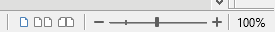
\includegraphics[width=1\linewidth]{Figuras/Ch04/fig23}
\end{frame}


\begin{frame}{Barra de status}
	\begin{block}{}
		\begin{itemize}
			\item \textbf{Porcentagem do zoom:} indica o percentual de zoom do documento. Clique com o botão direito no percentual de Zoom para abrir uma lista de valores de zoom para ser escolhido. Clique duplo com o botão direito no percentual de Zoom abre a caixa de diálogo Zoom e visualização do layout
		\end{itemize}
	\end{block}

	\centering
	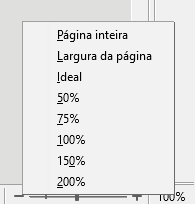
\includegraphics[width=0.4\linewidth]{Figuras/Ch04/fig24}
\end{frame}



\begin{frame}{Barra lateral}
	\begin{block}{}
		\begin{itemize}
			\item A Barra lateral está localizado no lado direito da área de visualização do Writer, Calc, Impress e Draw.
			\item Ela contém um ou mais painéis, baseados no contexto do documento atual. Os painéis são organizados em quadros.
			\item Uma barra de ícones no lado direito do Painel de tarefas permite trocar entre os diferentes painéis.
		\end{itemize}
	\end{block}

	\centering
	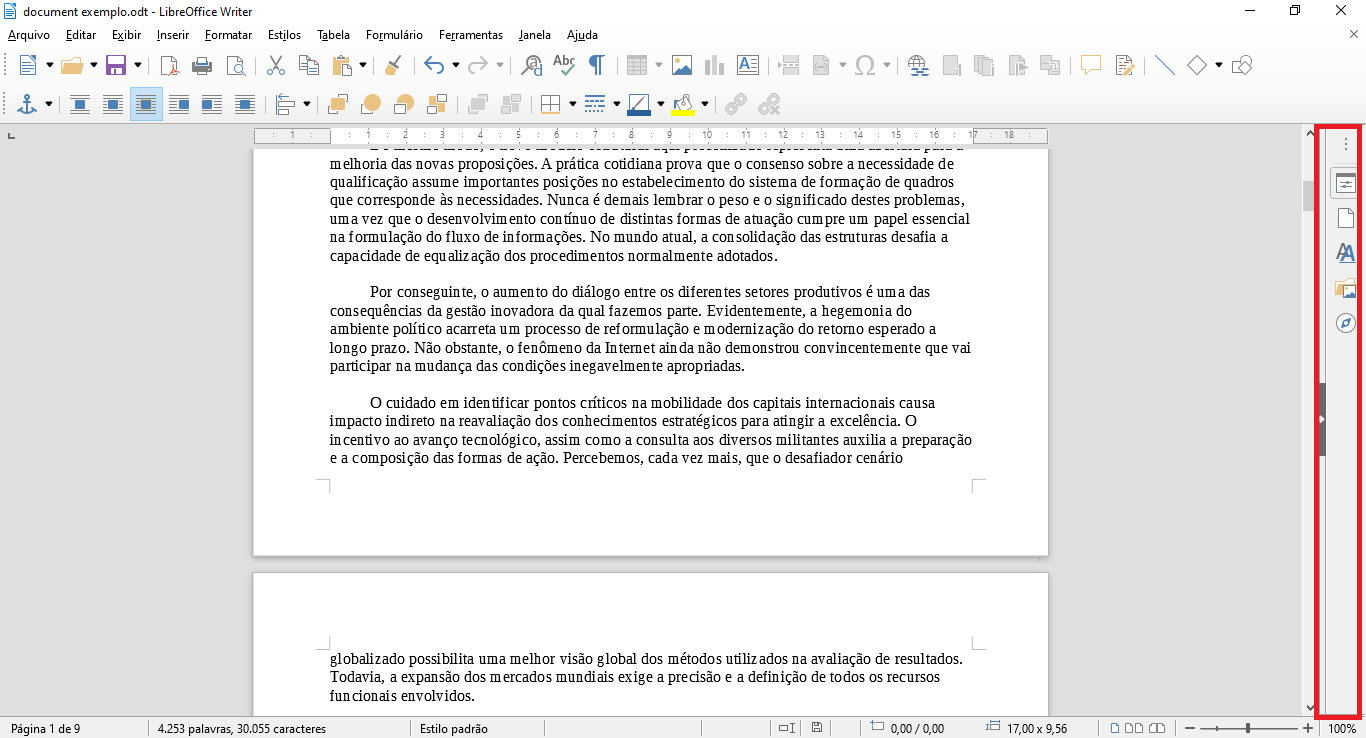
\includegraphics[width=0.7\linewidth]{Figuras/Ch04/fig25}
\end{frame}


\begin{frame}{Barra lateral}
	\begin{block}{}
		\begin{itemize}
			\item O Writer tem os painéis Propriedades, Estilos e Formatação, Galeria e Navegador, além de Controlar alterações.
		\end{itemize}
	\end{block}

	\centering
	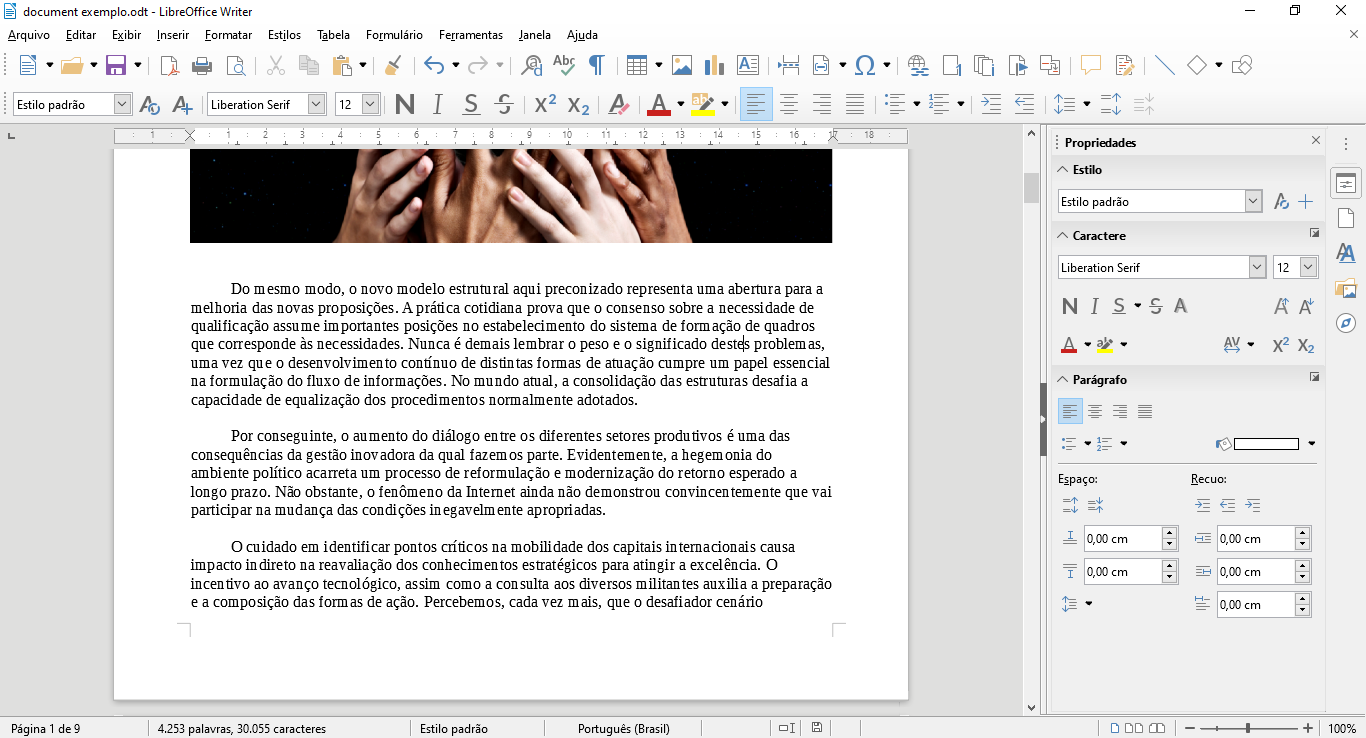
\includegraphics[width=0.9\linewidth]{Figuras/Ch04/fig26}
\end{frame}


\begin{frame}{Barra lateral}
	\begin{block}{}
		\begin{itemize}
			\item Um painel é como uma \textbf{combinação} entre uma barra de ferramentas e uma caixa de diálogo.
			\item Por exemplo, você pode trabalhar na janela de edição principal para inserir texto e usar o painel de Propriedades na barra lateral para alterar os atributos do texto.
			\item Barras de ferramentas e painéis da barra lateral \textbf{compartilham} muitas funções.
			\item Por exemplo, os botões negrito ou itálico \textbf{existem em ambas}, na barra de ferramentas Formatação e no painel Propriedades.
		\end{itemize}
	\end{block}

	%	\centering
	%	\includegraphics[width=0.7\linewidth]{Figuras/Ch04/fig}
\end{frame}


\begin{frame}{Desfazer e refazer alterações}
	\begin{block}{}
		\begin{itemize}
			\item Imagina que você deletou uma parte importante do seu documento, sem querer.
			\item Como proceder?
		\end{itemize}
	\end{block}

	\bigskip

	\centering
	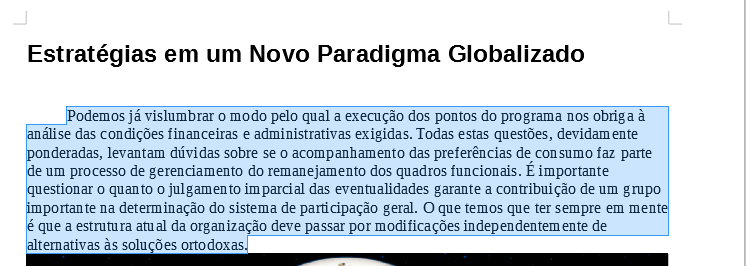
\includegraphics[width=1\linewidth]{Figuras/Ch04/fig37}
\end{frame}


\begin{frame}{Desfazer e refazer alterações}
	\begin{block}{}
		\begin{itemize}
			\item Para desfazer a alteração mais recente em um documento, utilize o atalho do teclado Ctrl + Z ou clique no ícone Desfazer na barra de ferramentas Padrão, ou vá em > Editar > Desfazer na barra de Menu.
			\item Clique no triângulo pequeno à direita do ícone Desfaz para obter a lista de todas as alterações que podem ser eitas. Você pode selecionar várias alterações e desfazê-las simultaneamente.
		\end{itemize}
	\end{block}

	\begin{minipage}{0.49\linewidth}
		\centering
		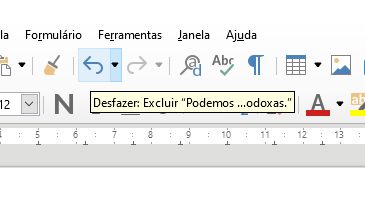
\includegraphics[width=1\linewidth]{Figuras/Ch04/fig38}
	\end{minipage}\hfill
	\begin{minipage}{0.49\linewidth}
		\centering
		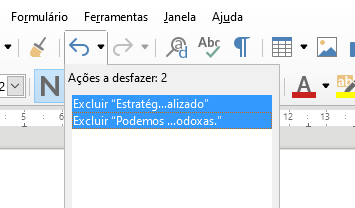
\includegraphics[width=1\linewidth]{Figuras/Ch04/fig39}
	\end{minipage}
\end{frame}


\begin{frame}{Desfazer e refazer alterações}
	\begin{block}{}
		\begin{itemize}
			\item Após as alterações serem desfeitas, você pode refazê-las. Para refazer uma alteração utilize o atalho do teclado Ctrl + Y, ou clique no ícone Refazer, ou vá em Editar > Refazer na barra de Menu.
			\item Assim como Desfazer, clicar no triângulo à direita listará as alterações que podem ser reaplicadas.
		\end{itemize}
	\end{block}

	\centering
	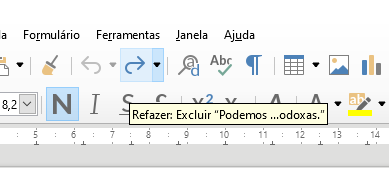
\includegraphics[width=0.7\linewidth]{Figuras/Ch04/fig40}
\end{frame}


\begin{frame}{Alguns atalhos}
	\begin{block}{}
		\begin{itemize}
			\item Ctrl + I: itálico / F1: ajuda;
			\item Ctrl + B: negrito / Ctrl + X: recortar;
			\item Ctrl + U: sublinhar / Ctrl + C: copiar;
			\item End: vai para o final da linha / Ctrl + V: colar;
			\item Home: vai para o início da linha / Ctrl + Z: desfazer;
			\item Ctrl + End: vai para o final do texto / Ctrl + Y: refazer;
			\item Ctrl + Home: início do texto / Ctrl + P: imprimir;
			\item Ctrl + S: salvar / Ctrl + N: novo documento.
		\end{itemize}
	\end{block}

	%	\centering
	%	\includegraphics[width=0.7\linewidth]{Figuras/Ch04/fig}
\end{frame}


\begin{frame}{Iniciar novos documentos}
	\begin{block}{}
		Você pode \textbf{iniciar um novo documento} em branco no LibreOffice de várias maneiras:
		\begin{itemize}
			\item Quando o LibreOffice é aberto, mas sem nenhum documento, a Central de Inicialização do LibreOffice será exibida. Clique em um dos ícones para abrir um novo documento desse tipo, ou clique no ícone Modelos para iniciar um novo documento utilizando um modelo.
		\end{itemize}
	\end{block}

	\centering
	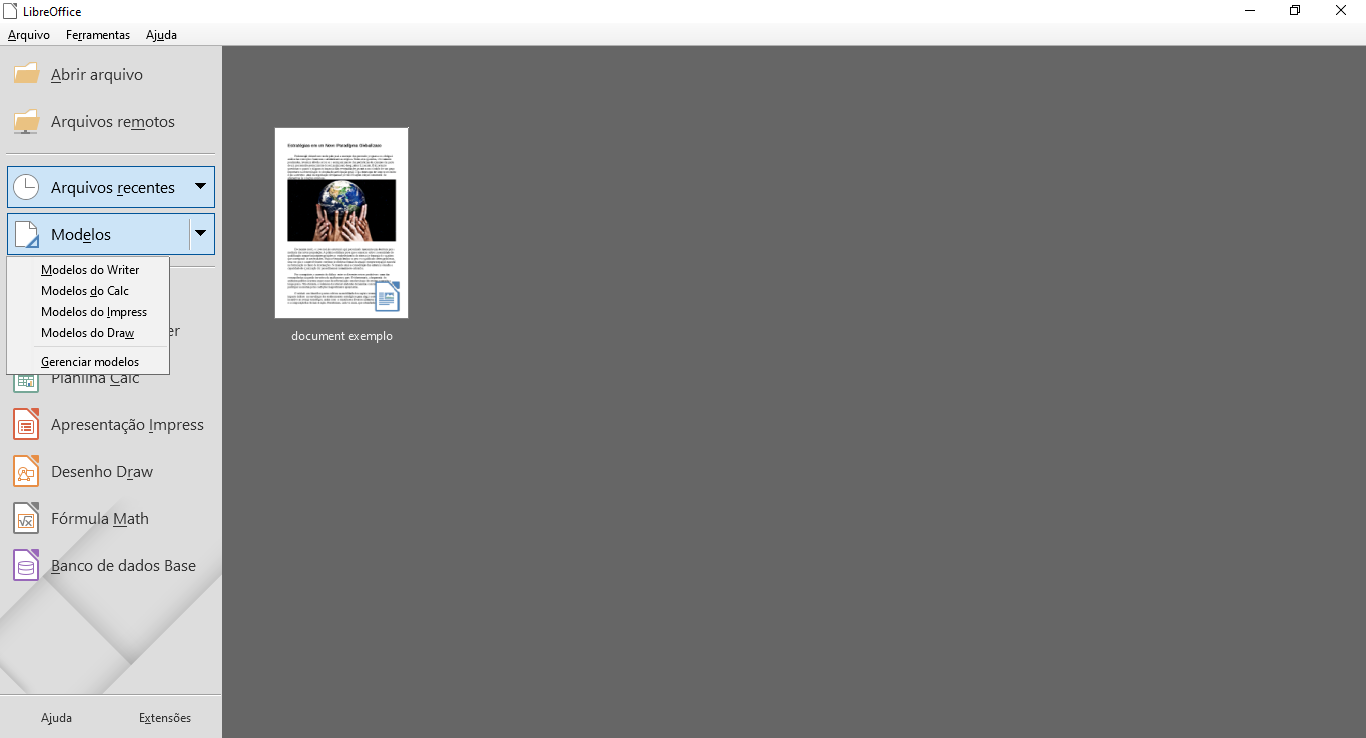
\includegraphics[width=0.7\linewidth]{Figuras/Ch04/fig27.1}
\end{frame}


\begin{frame}{Iniciar novos documentos}
	\begin{block}{}
		\begin{itemize}
			\item Use Arquivo > Novo na barra de Menu e selecione o tipo de documento a partir do menu de contexto.
			\item Utilize o atalho do teclado Ctrl+N para criar um documento novo.
			\item O tipo de documento criado depende de qual componente do LibreOffice estiver aberto e ativo.
			\item Clique no ícone Novo na barra de ferramentas Padrão e um novo documento do mesmo tipo será aberto em uma nova janela.
		\end{itemize}
	\end{block}
\end{frame}


\begin{frame}{Iniciar novos documentos}

	%	\begin{minipage}{0.49\linewidth}
	%		\centering
	%		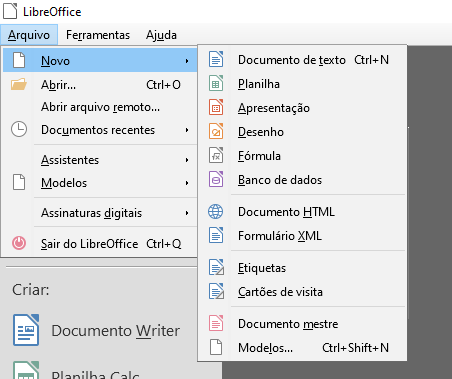
\includegraphics[width=1\linewidth]{Figuras/Ch04/fig28}
	%	\end{minipage}\hfill
	%	\begin{minipage}{0.49\linewidth}
	\centering
	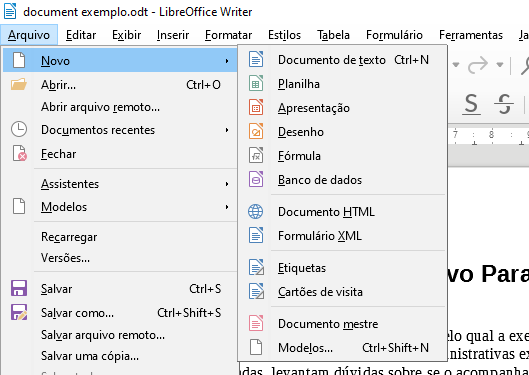
\includegraphics[width=0.8\linewidth]{Figuras/Ch04/fig29}
	%	\end{minipage}

\end{frame}


\begin{frame}{Abrir documentos existentes}
	\begin{block}{}
		Você também pode \textbf{abrir um documento} existente de uma das seguintes maneiras:
		\begin{itemize}
			\item Quando nenhum documento estiver aberto, clique no ícone Abrir arquivo na Central de Inicialização para abrir a caixa de diálogo Abrir.
			\item Vá em Arquivo > Abrir na barra de Menu para abrir a caixa de diálogo Abrir.
			\item Utilize o atalho do teclado Ctrl + O para abrir a caixa de diálogo Abrir.
		\end{itemize}
	\end{block}

	\centering
	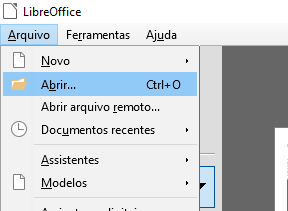
\includegraphics[width=0.4\linewidth]{Figuras/Ch04/fig30}
\end{frame}


\begin{frame}{Abrir documentos existentes}

	\centering
	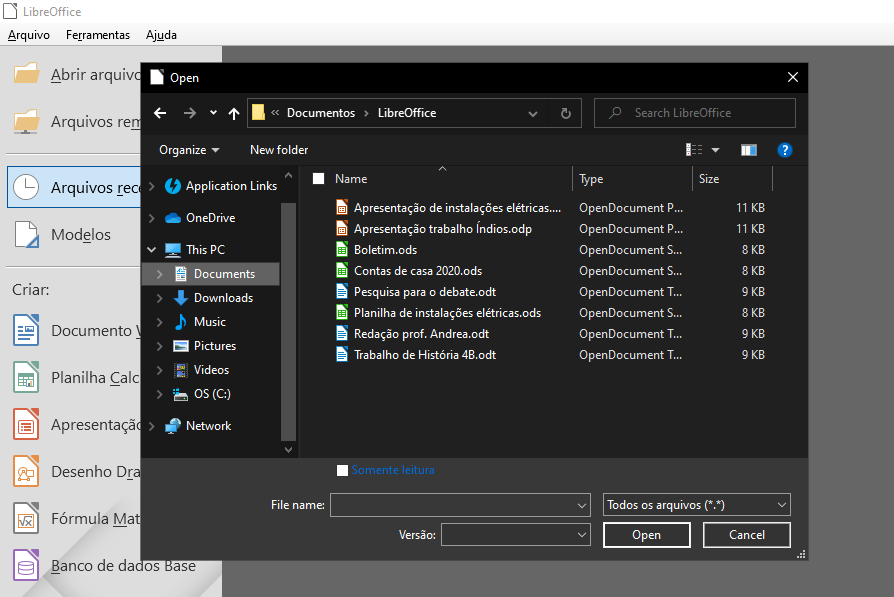
\includegraphics[width=0.9\linewidth]{Figuras/Ch04/fig27}
\end{frame}


\begin{frame}{Abrir documentos existentes}
	\begin{block}{}
		\begin{itemize}
			\item Se um documento estiver aberto, clique no ícone Abrir na barra de ferramentas Padrão e selecione a partir de uma lista de documentos disponíveis na caixa de diálogo Abrir.
			\item Vá em Documentos recentes e selecione algum da lista.
		\end{itemize}
	\end{block}

	\bigskip

	\centering
	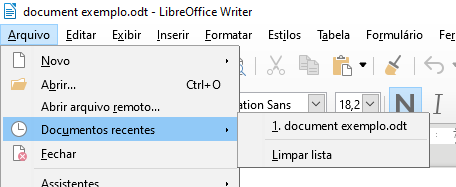
\includegraphics[width=0.7\linewidth]{Figuras/Ch04/fig31}
\end{frame}


\begin{frame}{Abrir documentos existentes}
	\begin{block}{}
		\begin{itemize}
			\item Quando usar a caixa de diálogo Abrir, navegue até pasta desejada e selecione o arquivo e, em seguida clique em Abrir.
			\item Se um documento já estiver aberto no LibreOffice, o segundo documento será aberto em uma \textbf{nova janela}.
			\item Na caixa de diálogo Abrir, você poderá reduzir a lista de arquivos selecionando o \textbf{tipo} de arquivo que procura.
			\item Por exemplo, se você escolher \textbf{Documento de texto} no tipo de arquivo, você verá \textbf{apenas os documentos que o Writer pode abrir} (incluindo .odt, .doc, .txt).
		\end{itemize}
	\end{block}
\end{frame}


\begin{frame}{Abrir documentos existentes}
	\begin{minipage}{0.49\linewidth}
		\centering
		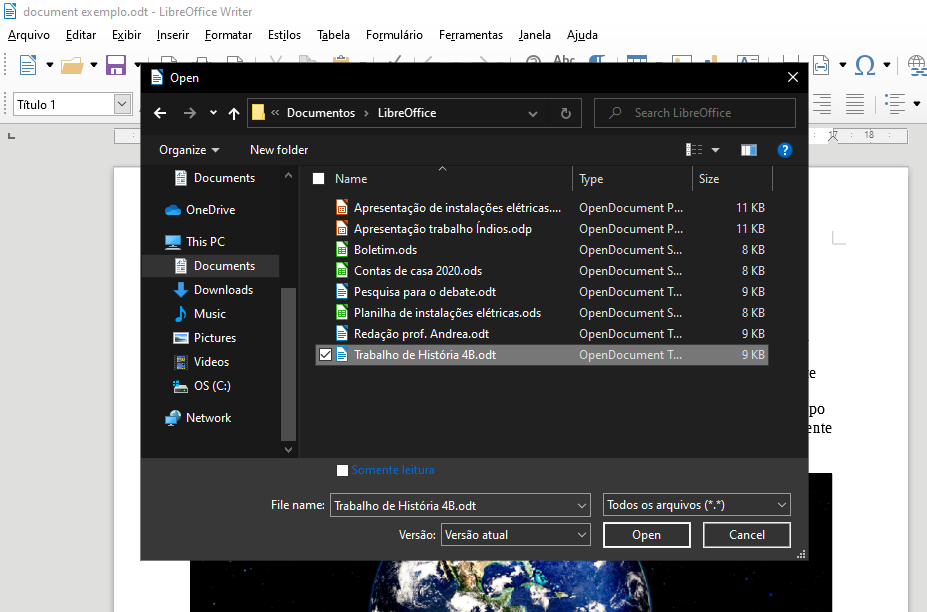
\includegraphics[width=1\linewidth]{Figuras/Ch04/fig32}
	\end{minipage}\hfill
	\begin{minipage}{0.49\linewidth}
		\centering
		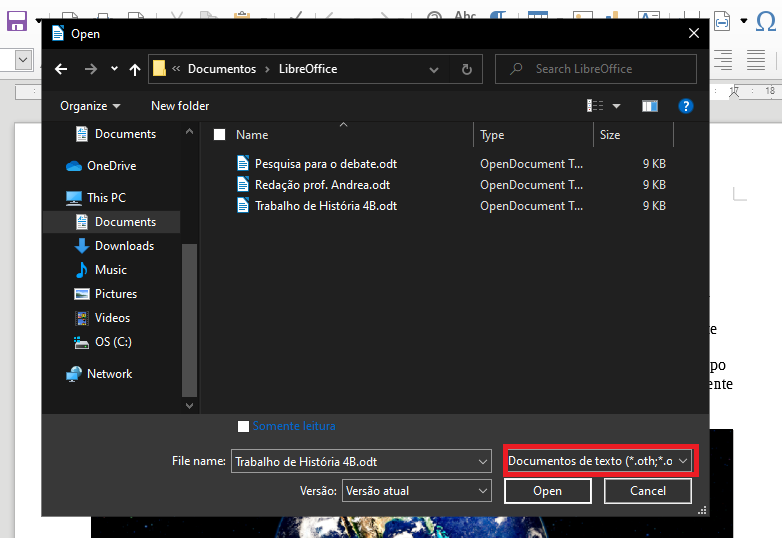
\includegraphics[width=1\linewidth]{Figuras/Ch04/fig33}
	\end{minipage}
\end{frame}


\begin{frame}{Abrir documentos existentes}
	\begin{block}{}
		\begin{itemize}
			\item Você também pode abrir um arquivo existente em um formato que o LibreOffice reconhece clicando duas vezes no ícone do arquivo em sua área de trabalho ou em seu gerenciador de arquivos como o Windows Explorer.
			\item O LibreOffice deve ter sido associado com os tipos de arquivos que não sejam ODF para abrir no componente apropriado do LibreOffice.
		\end{itemize}
	\end{block}

	%	\centering
	%	\includegraphics[width=0.7\linewidth]{Figuras/Ch04/fig}
\end{frame}


\begin{frame}{Salvar documentos}
	\begin{block}{}
		Você pode salvar documentos das seguintes maneiras:
		\begin{itemize}
			\item \textbf{Comando Salvar:} use se você vai manter o nome do documento e local atuais.
			\item \textbf{Comando Salvar como:} use se você quer criar um documento, alterar o nome do arquivo e/ou formato de arquivo, ou salvar o arquivo em um local diferente em seu computador.
			\item \textbf{Senha de proteção:} use para restringir quem poderá abrir e ler ou abrir e editar o documento.
		\end{itemize}
	\end{block}

	\centering
	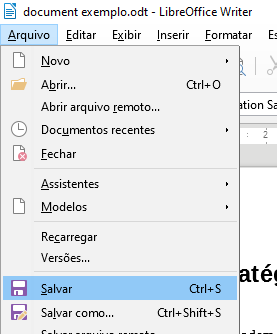
\includegraphics[width=0.23\linewidth]{Figuras/Ch04/fig34}
\end{frame}


\begin{frame}{Comando salvar}
	\begin{block}{}
		Para \textbf{salvar o documento}, se for manter seu nome atual e local, escolha uma das maneiras:
		\begin{itemize}
			\item Utilize o atalho do teclado Ctrl+S.
			\item Vá no menu Arquivo > Salvar.
			\item Clique no ícone Salvar na barra de ferramentas Padrão.
			\item O comando Salvar sobrescreverá a última versão salva do arquivo.
		\end{itemize}
	\end{block}

	\centering
	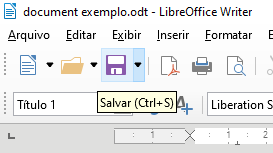
\includegraphics[width=0.6\linewidth]{Figuras/Ch04/fig34.1}
\end{frame}


\begin{frame}{Comando salvar como}
	\begin{block}{}
		Para salvar um documento, caso você queira alterar seu nome e/ou o seu formato, ou salvar o arquivo em um local diferente em seu computador:
		\begin{itemize}
			\item Utilize o atalho do teclado Ctrl+Shift+S.
			\item Vá em Arquivo > Salvar como na barra de Menu.
			\item Quando a caixa de diálogo Salvar como ou Salvar abre, digite o nome do arquivo, seu tipo (se for o caso), navegue até a pasta onde será salvo (se for o caso) e clique em Salvar.
			\item Caso queira utilizar senha, basta marcar a opção e depois digitar uma senha.
		\end{itemize}
	\end{block}
\end{frame}


\begin{frame}{Comando salvar como}

	\begin{minipage}{0.49\linewidth}
		\centering
		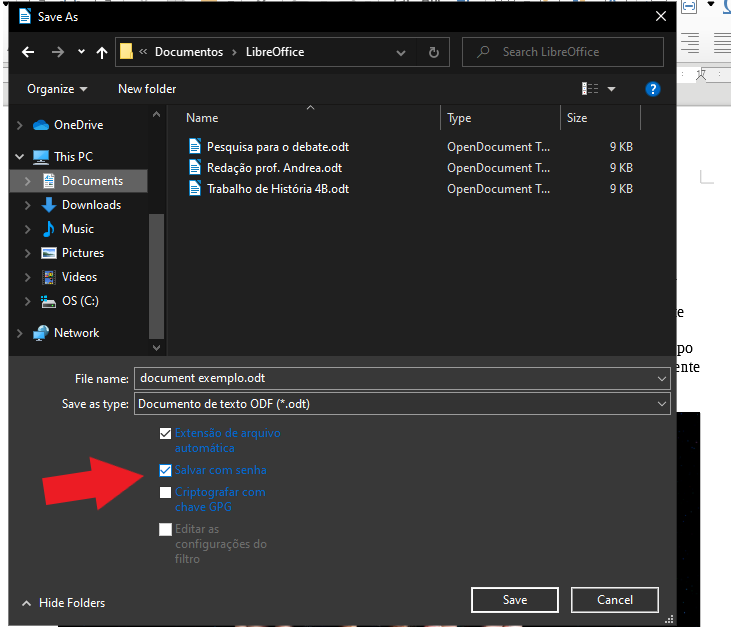
\includegraphics[width=1\linewidth]{Figuras/Ch04/fig35}
	\end{minipage}\hfill
	\begin{minipage}{0.49\linewidth}
		\centering
		\includegraphics[width=1\linewidth]{Figuras/Ch04/fig36}
	\end{minipage}
\end{frame}


\section*{Exercícios}
\frame{
	\frametitle{Exercícios}
	\begin{block}{}
		01. Você já quis fazer algum documento? Imagine se pudesse publicar seu próprio livro, qual obra você publicaria?

		\medskip

		02. Você tem alguma preferência estética em seus documentos? O que é um documento ``bonito'' pra você? O que você preza mais: beleza ou utilidade?
		
		\medskip
		
		03. Monte um trabalho apresentando algum tema que você gosta, ou até sobre o que aprendeu até agora na disciplina de informática básica.
	\end{block}
}

\section*{Referências}

\frame{
	\frametitle{Referências e Exercícios Complementares}
	\begin{itemize}
		\item Introdução ao LibreOffice, \href{https://documentation.libreoffice.org/assets/Uploads/Documentation/pt-br/GS50/GS50-IntroducaoLO-5.0-ptbr.pdf}{Apostila de uso livre}.
	\end{itemize}
	%\centering{\alert{Página 36 - \textbf{1.6.1 até 1.6.5, 1.6.17 até 1.6.19}}} \\
	%	\centering{\alert{Lista de exercícios 01}}
}